\documentclass[doc]{apa6}

\usepackage[english]{babel}
\usepackage[utf8x]{inputenc}
\usepackage{amsmath}
\usepackage{graphicx}
\usepackage{apacite}
\usepackage{amsfonts}
\usepackage{url}
\usepackage{tikz}
\usepackage{subfigure}
\usetikzlibrary{bayesnet}
\usepackage{bm}

%\usepackage[style=apa,sortcites=true,sorting=nyt,backend=biber]{biblatex}
%\DeclareLanguageMapping{american}{american-apa}

  \title{Big \emph{for a what}? Inferring comparison classes for relative adjectives}
    \author{Michael Henry Tessler\textsuperscript{1} and Noah D. Goodman\textsuperscript{1}}
    \date{}
  
\shorttitle{ Inferring comparison classes}
\affiliation{
\vspace{0.5cm}
\textsuperscript{1} Department of Psychology, Stanford University}
\keywords{comparison class; pragmatics; Rational Speech Act; Bayesian cognitive model; Bayesian data analysis\newline\indent Word count: X}
\makeatletter
\newcommand\LastLTentrywidth{1em}
\newlength\longtablewidth
\setlength{\longtablewidth}{1in}
\usepackage{tabularx}
\usepackage{multicol}
\usepackage{wrapfig}
\usepackage{gensymb}
\usepackage{tikz}
\usepackage{caption}
\usepackage{booktabs}

\authornote{Complete departmental affiliations for each author
(note the indentation, if you start a new paragraph). Enter author note
here.

Correspondence concerning this article should be addressed to Michael
Henry Tessler, 450 Serra Mall, Bldg. 420, Rm. 316, Stanford, CA 94305.
E-mail:}

\abstract{
The meaning of an utterance can change depending on the context. Yet,
what counts as the relevant context is often only implicit in everyday
conversation. The utterance ``it's warm outside'' signals that the temperature outside is relatively high, but the temperature could be high relative to a number of different \emph{comparison classes}:  warm
relative to other days of the year, warm for the season, warm for the week, etc.. 
Theories of context-sensitive language use agree that the comparison class is a crucial feature of meaning understanding, but little is known about how a listener reasons through this open-ended inference problem.
We present free-production and forced-choice experiments showing reliable patterns of comparison class inference.
The patterns of inference we observe are consistent with a model of Bayesian reasoning about the likely comparison class, which we incorporate into a probabilistic model of adjective interpretation, furthering the breadth of computational models of language understanding. 
The methods and results we present open the door to studying richer aspects of context-sensitive language understanding.
%We test the qualitative predictions of the model in a free production experiment and use a forced-choice version of the task to test the finer-grained, quantitative predictions. 
%The resolution of a comparison class requires not only reasoning about what is likely to be the case but also what would be informative to talk about, thus incorporating comparison class inference into the larger study of pragmatic reasoning.
}



\begin{document}
\maketitle

\definecolor{Red}{RGB}{255,0,0}
\definecolor{Green}{RGB}{10,200,100}
\definecolor{Blue}{RGB}{10,100,200}
\definecolor{Orange}{RGB}{255,153,0}

\newcommand{\denote}[1]{\mbox{ $[\![ #1 ]\!]$}}
\newcommand*\diff{\mathop{}\!\mathrm{d}}
\newcommand{\red}[1]{\textcolor{Red}{#1}}  
\newcommand{\ndg}[1]{\textcolor{Green}{[ndg: #1]}}  
\newcommand{\mht}[1]{\textcolor{Blue}{[mht: #1]}}  
\newcommand{\mlb}[1]{\textcolor{Orange}{[mlb: #1]}}

\section{Introduction}

A 75\degree F (24\degree C) day is warm. A 60\degree F (16\degree C) day is not. That is, unless it's January; 60\degree F could be warm for January. \emph{Warm} is a relative adjective, and its felicity depends upon what the speaker uses as a basis of comparison---the \emph{comparison class} (e.g., other days of the year or other days in January). Comparison classes are necessary for understanding relative adjectives and, in fact, any part of language whose meaning must be pragmatically reconstructed from context, including vague quantifiers \cite<e.g., ``He ate a lot of burgers.'';>{Scholler2017} and generic language \cite<e.g., ``Dogs are friendly'';>{Tessler2019psychrev}. Deciding on the relevant comparison class is a case study in the larger question of inferring the appropriate aspects of context for interpreting an utterance.  The trouble is: Comparison classes, as with relevant aspects of context more generally, often go unsaid (e.g., in ``It's warm outside'').

The existence of comparison classes for understanding relative adjectives is
uncontroversial \cite{cresswell1976semantics, klein1980semantics, kennedy2005scale, bale2008universal, Bale2011, Solt2009}. %\red{more standard citations for this?}
Adult judgments of the felicity for adjectives like \emph{dark} or \emph{tall} depend
upon fine-grained details of the statistics of the comparison class:
When objects in the comparison class are all rather short, what counts
as \emph{tall} might not be very tall \cite{Qing2014, Schmidt2009, Solt2012}.
Four-year-olds use their knowledge of kinds to differentiate between
what goes into the comparison class and what does not: What counts as a
\emph{tall pimwit} depends on the distribution of heights of
\emph{pimwits} and not the heights of other creatures like \emph{daxes}
\cite{Barner2008}. Even children as young as 2-and-a-half
understand that \emph{big} is relative \cite{Sera1987} and even that the
comparison class can change \cite<e.g., an objectively small mitten can be \emph{big} relative to the tiny mittens on the table;>{Ebeling1988, Ebeling1994}.

A speaker's choice of noun phrase can strongly influence the comparison class  (e.g., \emph{tall pimwits} are tall relative to other pimwits), though it need not determine it: ``That's a big snowman'' said to a 4-year-old might mean \emph{big relative to snowmen a 4-year-old could build} \cite{kamp1975two}.  
The major problem in determining the comparison class is that any particular referent of discourse can be conceptualized or categorized in
multiple ways, giving rise to multiple possible comparison classes. A day in
January is also a day of the year; if a listener hear ``It's
warm'', it could be \emph{warm for the week}, \emph{warm for winter}, or
\emph{warm for the year}.\footnote{It could also be \emph{warm for
  Boston}, \emph{warm for the northeast USA}, \emph{warm for a place
  with currently six inches of snow on the ground}, among many more
  possibilities. } In this paper, we investigate the first aspect of
this open-ended inference problem, deciding among multiple possible comparison
classes. Theoretical work in semantics has focused on how information
from the comparison class gets integrated with a compositional semantics
and what representations might be preferred \cite{Bale2011, Solt2009}.
The question of how listeners decide upon a comparison class when it's not stated explicitly (e.g., ``It's warm relative to other days this winter'') has been addressed neither formally nor empirically.

%Intuitively, the comparison class is not a fixed property of the referent nor the referent--predicate pair. 
%A ``tall basketball player'' might be tall for a basketball player or just tall for a person. 
An intuitive null hypothesis about how comparison classes are determined is that listeners perform a kind of Bayesian inference over the likely comparison class intended by the speaker, by balancing the probability that a speaker would use the adjective to describe the referent given a comparison class with the \emph{a priori} probability of a comparison class.
We explore such a hypothesis in this paper.
The prior distribution is over comparison classes is a theoretical object of interest in its own right, and we will only be able to begin to understand this distribution's properties via our experiments and model.%  of a comparison class is a 
But even given plausible values for the prior probabilities of comparison classes, this proposal predicts that when an adjective signals a degree (e.g., temperature) that is \emph{a priori} consistent with the listener's knowledge of the referent (e.g., as a member of a category that generally has a high or low temperature), the comparison class is likely to be a relatively general category (e.g., a basic or superordinate level category), whereas when the adjective signals a degree inconsistent with the listener's prior beliefs about the referent, the comparison class is likely to be a more specific (e.g., subordinate level) category.\footnote{Here, \emph{generally consistent} means generally high or low relative to a basic-level or superordinate level category that has some non-negligible probability of being a comparison class.}
For example, in Winter, hearing \emph{it's warm} should signal \emph{warm for winter} (subordinate comparison class), while hearing \emph{it's cold} signals \emph{cold for the year} (a more basic or superordinate class). 
The opposite relationship should hold in summer, where \emph{it's cold} should signal cold \emph{for summer} more so than \emph{it's warm}. 
We describe in detail the mechanism behind this inference, formalized in a probabilistic model of language understanding, which in turn generates quantitative predictions that depend on background knowledge about categories and their properties. 
We test the qualitative predictions in a large-scale free-production task where participants are asked to infer the comparison class the speaker had in mind. 
To generate quantitative predictions, we model a related language task with a structure similar to the comparison class inference experiment; this joint data modeling allows us to pin-down relevant model parameters that govern the prior knowledge in the cognitive model without having to ask participants difficult estimation questions often employed in eliciting prior knowledge for Bayesian cognitive models. 
We find that the comparison class can be flexibly adjusted based on prior knowledge, which our model can predict with high quantitative accuracy. 
\red{[zoom back out. bigger picture.]}
%This work provides 
%\red{We find X... [zoom back out. big picture] }

%This inference results from pragmatic reasoning and is not predicted by the alternative, non-pragmatic Bayesian model.
%These predictions fall out of a Rational Speech Act (RSA) model for gradable
%adjectives \cite{Lassiter2013, Lassiter2017}, extended to flexibly
%reason about the implicit comparison class. 

% a result of the \emph{a
%priori} probability of different temperatures in different seasons: In
%winter, temperatures are relatively low, and thus it is unlikely to
%actually be \emph{warm for the year}. 
%In addition, regardless of the
%season and the adjective (e.g., ``warm'' or ``cold''),
%listeners prefer comparison classes that are relatively specific (e.g.,
%relative to \emph{the current season} as opposed to \emph{the whole
%year}); more specific comparison classes have lower variance, and a
%vague adjectives like \emph{warm} carries more information when it is
%interpreted with respect to a lower variance comparison class. 

%\textcolor{Blue}{[mht: move to end of first expt]}
%
%The model's quantitative predictions can be generated by explicitly
%specifying the interlocutors' relevant prior knowledge (e.g., beliefs
%about temperatures). The current methodological standard is to measure
%beliefs by having participants estimate quantities or give likelihood
%judgments \cite{Franke2016}. We pursue a different methodology. The
%RSA model captures a productive fragment of natural language; thus, it
%makes predictions about a related natural language task (Expt. 2).
%Critically, we can use the model to predict natural language judgments
%that require the \emph{same prior knowledge} as in Expt. 1 and use
%Bayesian data analysis to jointly infer the shared priors. This approach
%harnesses the productivity of language into experiment design and allows
%us to reconstruct priors without having participants engage in
%challenging numerical estimation tasks.

\section{Computational Model}

We explicate our model with the example of hearing a basketball player described as \emph{tall} (Figure \ref{fig:modelCartoon}). 
The basic intuition that the model formalizes is that, when describing the height of a basketball player, a speaker is more likely to say \emph{he's a tall person} than \emph{he's a tall basketball player} because it is a more likely state of affairs given distributional knowledge of the heights of people and the heights of basketball players. 
A listener can use this knowledge to infer the unsaid comparison class when they hear only \emph{he's tall}.
The opposite inference is predicted when the basketball player is described as \emph{short} (i.e., more likely to be a \emph{short basketball player} than a \emph{short person}).
Finally, the same adjectives used to describe a jockey should invoke the opposite inferences (i.e., \emph{tall} $\rightarrow$ \emph{tall jockey}; \emph{short} $\rightarrow$ \emph{short person}).

Formally, a listener is faced with a joint inference problem of determining the height of the person $x$ and the comparison class  $c$ assumed by the speaker when producing their adjectival utterance $u$ (e.g., \emph{he's tall}).
We propose a Bayesian formulation to this problem, wherein a listener combines his prior knowledge about categories and what comparison classes are likely to be talked about with the likelihood that a speaker would use an adjective to describe a member of a particular category.\footnote{We use the male pronoun to refer to the listener and the female pronoun to refer to the speaker.}
The hypothesis space of comparison classes is constrained by  beliefs about the referent that are shared between the speaker and listener: A speaker is unlikely to be assuming a comparison class about which she has no knowledge.
%In our example, it is in common ground that the referent is a basketball player.
Though comparison classes can be constructed in various ways, including out of sets of objects in the perceptual environment or hypothetical functions of an object \cite<cf.,>{Ebeling1994}, we restrict our analysis to a hypothesis space of comparison classes constructed out of a taxonomic hierarchy of the subordinate category to which the referent belongs (i.e., \emph{conceptual comparison classes}, e.g., a basketball player is a person; Figure \ref{fig:modelCartoon}A).
In contrast to the space of comparison classes, the hypothesis space of degrees (e.g., heights) is informed by the totality of the listener's relevant beliefs (i.e., including both the shared beliefs with the speaker and the listener's private beliefs).
Though we distinguish formally between the beliefs of the speaker and listener, in the contexts we consider, it can be assumed that all relevant beliefs are shared beliefs; in our example, the listener knows that the referent is a basketball player, and hence would expect a height of the referent consistent with their knowledge of basketball players.

%For both of these random variables, the listener can employ knowledge to constrain the inference problem. 
%Specifically, 

%\begin{figure}[ht]
%  \begin{center}
%    \begin{tabular}{cc}
%\begin{tikzpicture}
%
%  % Define nodes
%  \node[latent]                             (u) {$u$};
%  \node[latent, above=of u, xshift=-1.2cm] (c) {${c}$};
%  \node[latent, above=of u, xshift=1.2cm]  (x) {${x}$};
%  \node[latent, above=of c, xshift=0cm] (f) {${f}$};
%  \node[latent, above=of x, xshift=0cm] (g) {${g}$};
%
%  % Connect the nodes
%  \edge {c,x} {u} ; %
%  \edge {f} {c} ; %
%  \edge {f,g} {x} ; %
%
%
%\end{tikzpicture}
%
%    \end{tabular}
%  \end{center}
%  \caption{Generative model of utterances in the mind of a listener. An utterance $u$ is a function of a comparison class $c$ and degree $x$, via the $S_2$ model (Equation \ref{eq:S2}). A listener's best guess about the degree is a function of both the shared beliefs about the referent $f$ and  the listener's private beliefs $g$. The comparison class $c$ is a function of only the shared beliefs between speaker and listener $f$.}
%  \label{fig:bayesnet}
%\end{figure}

A listener $L_n$ updates their beliefs about the degree $x$ and the comparison class $c$ by assuming that a speaker $S_n$ intentionally produced an adjectival utterance $u$ in order to communicate about the degree (e.g., height).
Formally, this inference can be captured in a Bayesian formulation:

\begin{align}
L_n(x, c \mid u, f, g) &\propto S_n(u \mid x, c) \cdot P(x \mid f, g) \cdot P(c \mid f) \label{eq:L2} 
\end{align}

\noindent where $f$ denotes the beliefs shared between speaker and listener, and $g$ denotes the listener's private beliefs. Since our paradigm does not distinguish between these kinds of beliefs, we use a reduced-form of the model, where beliefs are represented by a single variable $k$ and can be thought of as relevant category information about the referent (e.g., the referent is a basketball player): 

\begin{align}
L_n(x, c \mid u, k) &\propto S_n(u \mid x, c) \cdot P(x \mid k) \cdot P(c \mid k) \label{eq:L2} 
\end{align}

Following work in the Rational Speech Act modeling framework \cite{Frank2012, Goodman2016, scontras2017probabilistic}, the speaker $S$ in this model is a soft-max rational agent (with degree of rationality $\alpha$) who produces utterances in order to convey information to a listener $L$ who knows the comparison class, while also taking into account the cost of the utterance $u$.\footnote{For all of our quantitative and quantitative modeling, we assume no difference in production cost for different utterances. Hence, our model reduces to simply: $S_n(u \mid x, c) \propto L_{n-1}(x \mid u, c)^{ \alpha}$}


\begin{figure}
\centering
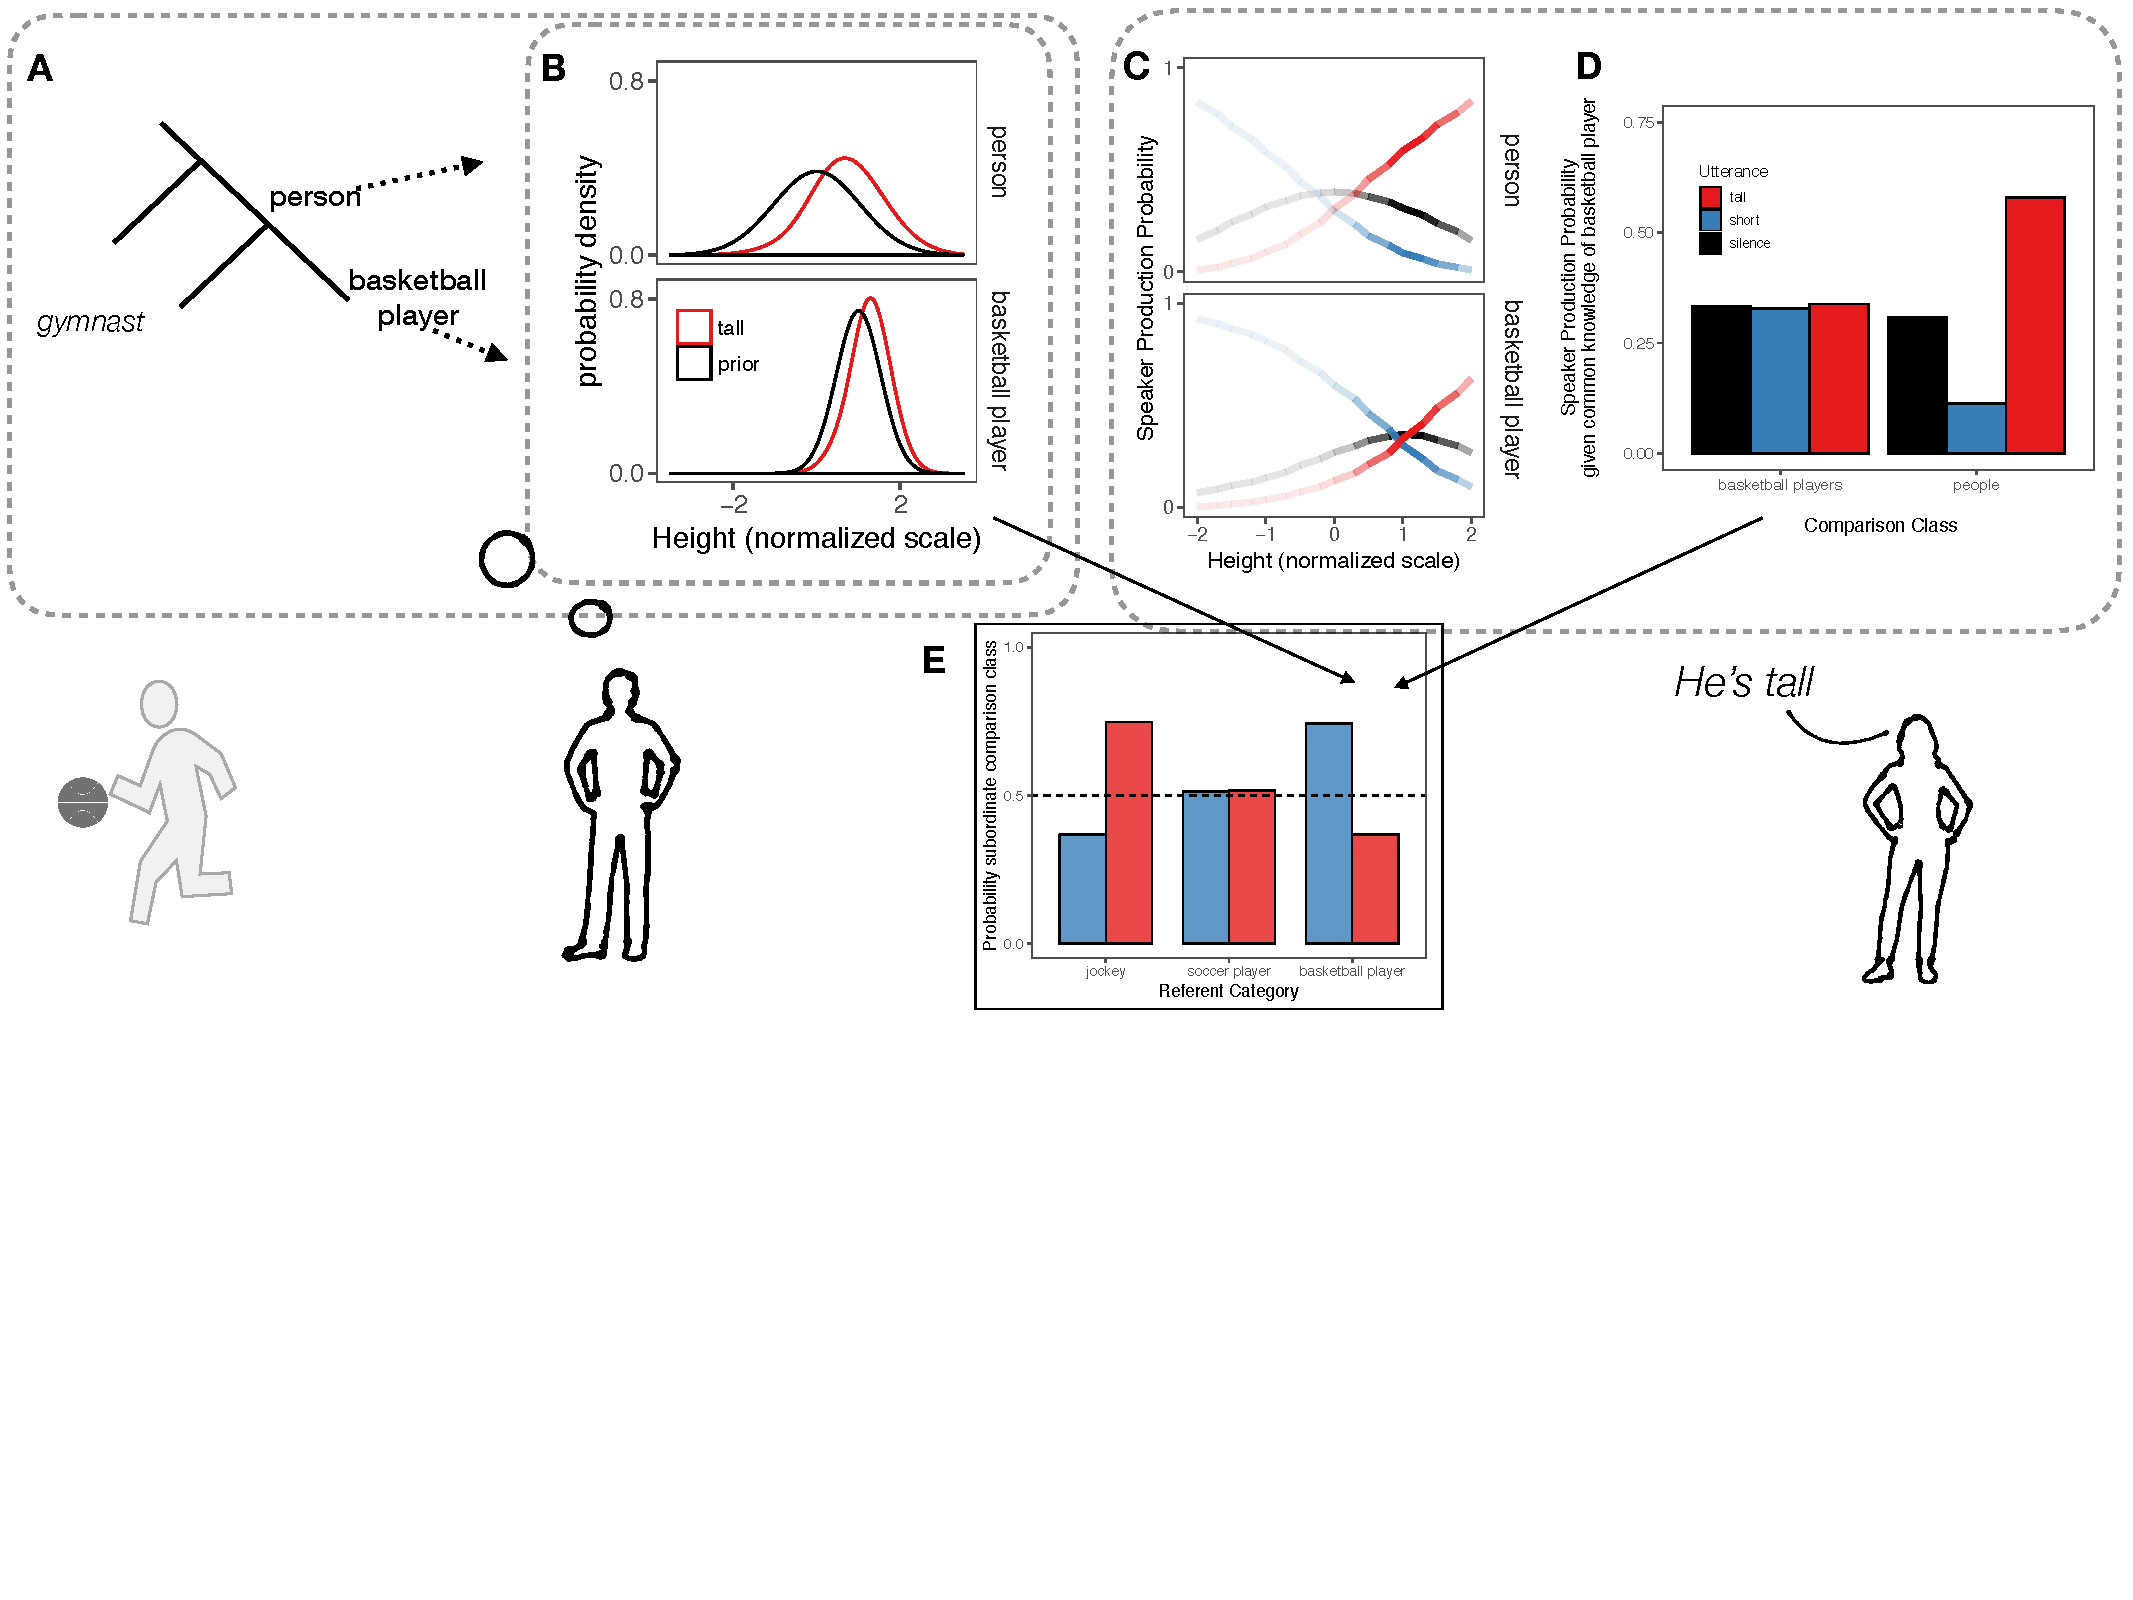
\includegraphics[width=\textwidth]{figs/model_cartoon.pdf}
\caption{\label{fig:modelCartoon}Model overview. A: A hypothesis space of comparison classes is constructed over a taxonomic hierarchy. B: A specific comparison class is realized as a probability distribution over the relevant degree (e.g., height; shown in black). The interpretation of a gradable adjective (e.g., \emph{tall}; shown in red)---given by $L_{n-1}(x \mid u, c)$---is sensitive to the comparison class. C: Listener $L_n$ imagines what a speaker $S_n$ would say given different comparison classes (facets) and assuming different possible heights of the referent (x-axis); the intensity of the colors (alpha/opacity) is in proportion to the listener's expectation of that particular height (e.g., the listener knows the referent is a basketball player, and so expects heights towards the upper range of the scale). D: Distribution of speaker utterances for different comparison classes marginalizing over the plausible heights of the referent. A speaker is more likely to say \emph{tall} is the comparison class is \emph{people}. E: Comparison class inference by the listener in terms of the probability of a subordinate class (e.g., basketball players) computed by inverting the speaker model. Listener is more likely to infer \emph{basketball players} as the comparison class when the referent is described as \emph{short} than when they are described as \emph{tall}.
% speaker production probability distributions are shown with the.
}
\end{figure}


\begin{align}
S_n(u \mid x, c) &\propto \exp{(\alpha \cdot (\ln L_{n-1}(x \mid u, c) - \text{cost}(u) ))}\label{eq:S2} 
\end{align}
%exp{(\alpha_1 \cdot \ln {L_{0}(x \mid u, \theta)} )}

We assume the speaker has three utterances she can say: \{\emph{tall}, \emph{short}, silence\}, where silence is a semantically vacuous utterance (i.e., a null action). 
The listener who updates their beliefs about the temperature given a vague adjectival utterance and a fixed comparison class $L_{n-1}(x \mid u, c)$ is model of context-sensitive adjective interpretation, a problem which has garnered a lot of recent attention by formal models of language understanding \cite{Lassiter2013, Qing2014a, Lassiter2017}.
Our model of comparison class inference builds on top of these formal theories, and we treat this model component $L_{n-1}(x \mid u, c)$ as a black-box function that produces a probability distribution over degrees (e.g., heights) in a manner that is sensitive to the comparison class (e.g., respecting the interpretative difference between \emph{tall person} and \emph{tall basketball player}; Figure \ref{fig:modelCartoon}B). 
%\red{Figure 1 shows the behavior of this model component.}
We adopt the model of \citeA{Lassiter2013, Lassiter2017} which, following standard treatment in formal semantics \cite<e.g.,>{Kennedy2007}, takes the literal meaning of a gradable adjective to be simply a threshold function on the degree (e.g., \([\![tall]\!] = height > \theta\)), where a pragmatic reasoning agent analogous to the speaker and listener models defined above reasons about the plausible threshold the speaker is using, given their knowledge of the comparison class.\footnote{Following standard treatment of antonyms, the
  semantics of \emph{short} are a threshold function on a distinct
  threshold variable: \([\![u_{short}]\!] = height < \theta_{short}\)), which
  is also inferred via the pragmatic listener (i.e., the listener infers
  a threshold for both \emph{tall} and \emph{short}). The pragmatic
  inferences about the comparison class that are the focus of this paper
  are invariant to whether or not the antonym is included in the
  alternative set. The comparison class inferences are also invariant to
  whether or not the antonym gets assigned its own unique threshold
  (\(\theta_{short}\)).}
  A full presentation of this  part of the model is given in Appendix A.
  
We consider an idealized case where the comparison class can be either a relatively specific (subordinate-level, \(c_{sub}\)) or relatively general (basic-level, \(c_{basic}\)) categorization (e.g., tall relative to \emph{basketball players} or relative to \emph{people}): \(c \in \{c_{sub}, c_{basic}\}\).
To understand the model behavior, consider the speaker model \(S_n\) under different assumptions (by the listener) about the implicit comparison class: \(S_{n}(u \mid x, c = c_{sub})\) and \(S_{n}(u \mid x, c = c_{basic})\). 
Figure \ref{fig:modelCartoon}C shows the speaker production probabilities of the three possible utterances for each value along the degree scale (e.g., each height) for the two different comparison classes.  If the comparison class is \emph{people}, the speaker will produce \emph{tall} when the height of the referent is substantially greater than the average height for people, with the speaker more likely to say \emph{tall} as the height of the referent increases.
  If the comparison class is \emph{basketball players}, the speaker's criterion shifts to the right and she becomes more reluctant to produce \emph{tall} until the height of the referent is much greater (all utterance curves shift to the right). 
  The listener combines this generative model of adjectival utterances with their prior knowledge about the height of the referent: The listener knows the referent is a basketball player and thus their likely height is given by the basketball player distribution (Figure \ref{fig:modelCartoon}B, bottom, black; this distribution is superimposed as an opacity on Figure \ref{fig:modelCartoon}C).
  When the listener marginalizes over their beliefs in the height of the referent, the speaker is thought to be more likely to produce \emph{tall} if the comparison class were \emph{people} (Figure \ref{fig:modelCartoon}D).  

The listener inverts their generative model of the utterance (i.e., the speaker model) to infer the comparison class assumed (Figure \ref{fig:modelCartoon}E).
Because the speaker is more likely to stay \emph{tall} if the comparison class were \emph{people}, the listener reasons that a speaker who says \emph{tall} probably was assuming a more general comparison class (i.e., that the comparison class is \emph{people}). 
If, however, the listener hears of the basketball player that he is \emph{short}, the more likely comparison class is the subordinate class of \emph{basketball players}.
This inference is driven by prior knowledge about the category, and thus, we would expect the inferences to change if the prior knowledge changes.
Indeed, the same adjectives used to describe a member of a subordinate category that tends to fall low on the degree scale (e.g., jockeys, who tend to short people) will result in the opposite inferences about the comparison class. 
Thus, our model predicts that the comparison class can be flexibly adjusted and it provides a precise quantitative formulation in how this inference should be driven. 

%The utterance which does not reference a class (e.g., It's warm}) inherits the same meaning as the utterance with the explicit class that
%matches the assumed implicit class (i.e., if \(c_{i} = c_{sub}\), then
%\(u_i\) has the same meaning as \(u_{sub}\)). Therefore, reasoning about
%the likely comparison class reduces to reasoning about which explicit
%utterance the speaker would have been more likely to say.
  


\section{Overview of Experiments}

\begin{figure*}[htb]
{\centering 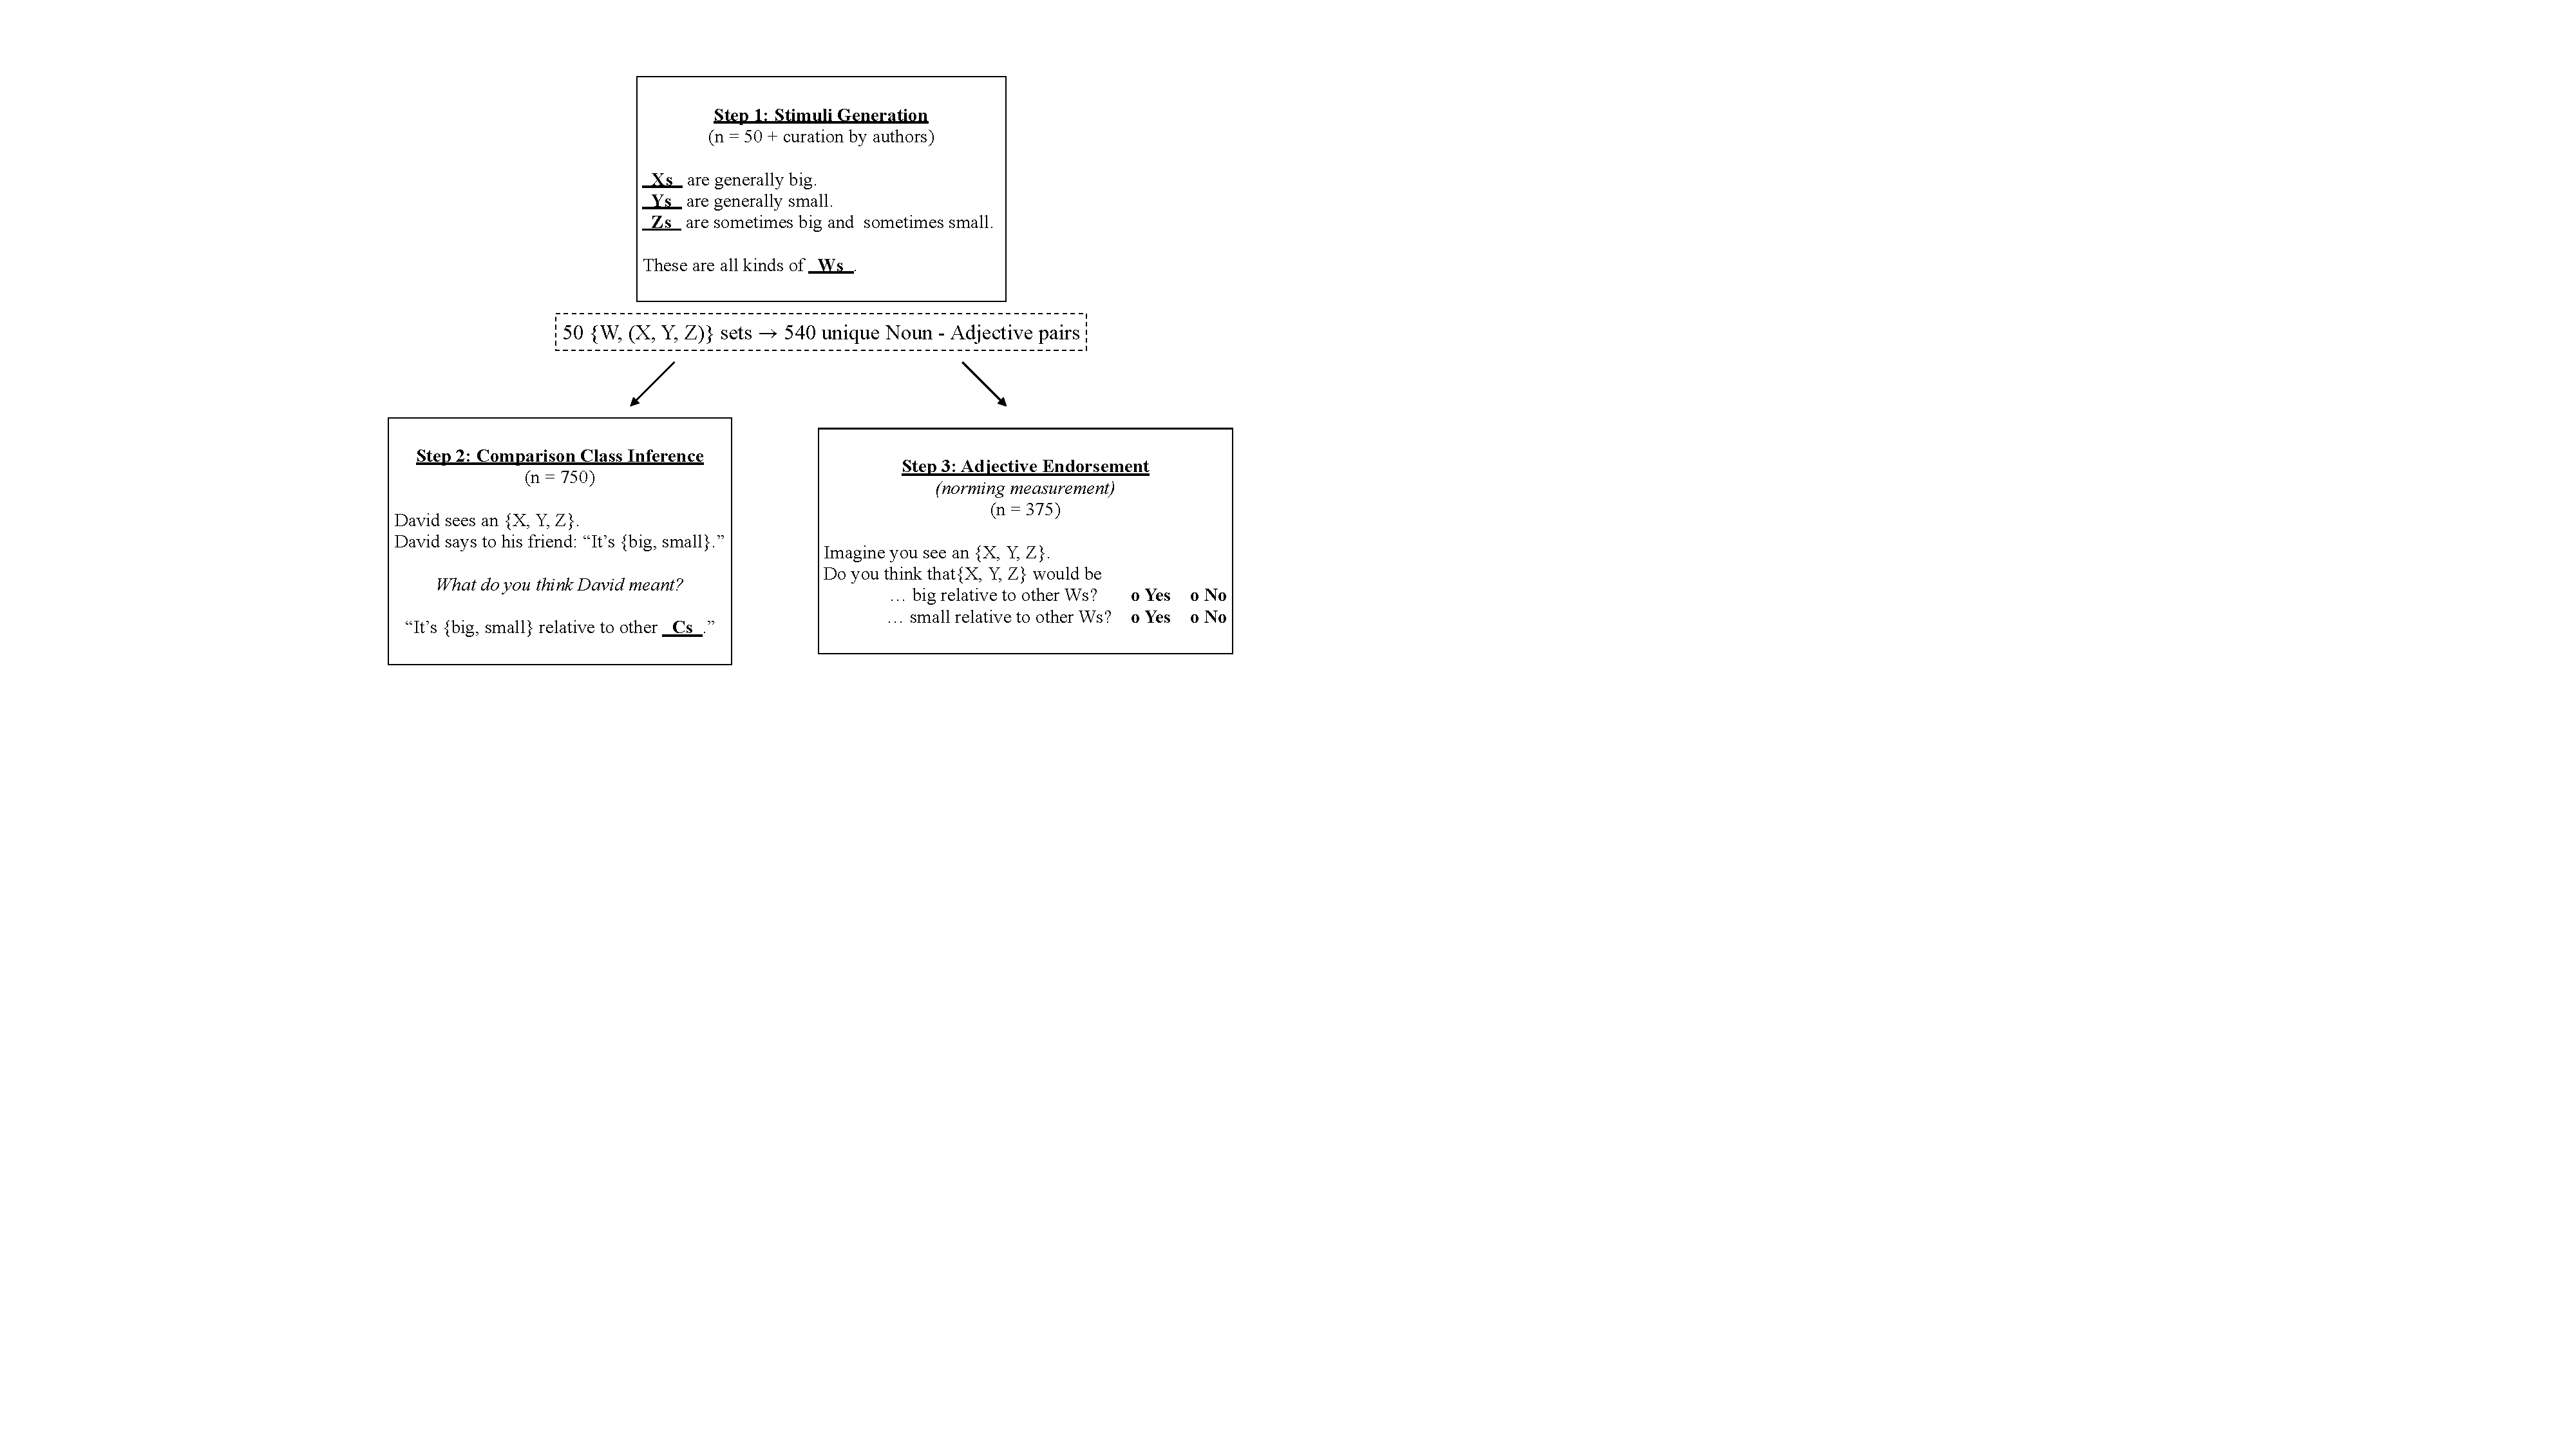
\includegraphics[width=1\textwidth]{figs/expt_overview} }
\caption{Overview of Experiments. Step 1: Using a structured production task, we elicit sets of stimuli that all share the feature of containing categories generally judged as having either a positive or negative adjective  (\emph{X, Y}; e.g., big or small) applied to them as well as a control category (\emph{Z}; e.g., sometimes big and sometimes small). The task is designed in a way to elicit three categories of the same basic- or superordinate-level category (\emph{W}). Step 2: Forced-choice task where participants judge whether a member of the subordinate level category would be judged as a having the adjective applied explicitly relative to the basic/superordinate level category. This task serves to validate our experimental stimuli as well as provide additional data to constrain the parameters of the comparison class inference model. Step 3: Free-production task to elicit the comparison class.}\label{fig:exptOverview}
\end{figure*}

We test our hypothesis the comparison class can be flexibly adjusted based on world knowledge and pragmatic principles in a set of coordinated experiments (Figure \ref{fig:exptOverview}).
We first empirically elicit test stimuli by having participants fill out phrasal templates that aim to elicit sets of categories at the same level of hierarchy that tend to be on extreme ends of a degree scale (e.g., categories that are generally big or generally small) as well as a control item (e.g., a category whose members are sometimes big and sometimes small; Step 1). 
We then validate these stimuli using a forced-choice paradigm where participants are asked to judge whether an adjective (e.g., \emph{big} or \emph{small}) would be true of a member of a subordinate category relative to the basic or superordinate category (Step 2). 
This adjective endorsement task also provides additional data to constrain the parameters of the comparison class inference model (described below).
Finally, we test the qualitative predictions shown in Figure \ref{fig:modelCartoon}E by having participants rephrase a speaker's statement in a way that makes the comparison class explicit (Step 3).
The quantitative predictions of the model are tested using a Bayesian data analytic strategy, where we explicitly model the data from both the Adjective Endorsement (Step 2) and Comparison Class Inference (Step 3) tasks jointly.
This joint Bayesian data-analytic strategy allows us to infer, rather than stipulate, the world knowledge that guides the inference about the comparison class in the computational model. 

\section{Data-analytic Strategy}

Our comparison class inference model makes qualitative predictions about the likely comparison class assumed by a speaker when they hear an adjective in isolation (e.g., \emph{he's tall}; Figure \ref{fig:modelCartoon}E). 
The model is a quantitative model, however, and can make quantitative predictions concerning the strength of comparison class inferences given model parameters that describe world knowledge $P(x)$ and prior expectations about the comparison class $P(c)$.
Previous modeling papers in the RSA tradition empirically elicit world knowledge through prior elicitation tasks.
These tasks often involve estimating numerical quantities or making probability judgments, for which complicated linking functions must be designed \cite{Franke2016}. 
We take a different approach: We make small modifications to the same core RSA architecture to make predictions about a related language task concerning the same domains used in the Comparison Class Inference task. 
We then construct a Bayesian data analytic model to infer the world knowledge shared between these two tasks, along with the few other free parameters of the model (Figure \ref{fig:bayesnet}). 
This \emph{descriptive Bayesian approach} \cite{tauber2017} coupled with explicit models of language understanding allow us to model broader coverage data sets while still constraining model flexibility by forcing the models to predict more distinct data points. 

In our model, world knowledge is represented by probability distributions over degrees (e.g., heights).
Because we simplify the problem to only considering two comparison classes---a subordinate class (e.g., basketball players) and a basic or superordinate class (e.g., people)---only the relative values for the degrees affect model predictions. 
Hence, we fix each basic/superordinate class in each domain to be a standard normal distribution---$P(x \mid c = c_{basic}) = \mathcal{N}(0, 1)$---and we assume the subordinate priors to also be Gaussian distributions---\(P(x \mid c = c_{sub}) = \mathcal{N}(\mu_{sub}, \sigma_{sub})\); the subordinate priors thus have standardized units.
We infer the plausible values of the parameters governing the subordinate priors from the data.

The data from the comparison class experiment would be insufficient, however, to reliably estimate the model parameters governing the world knowledge priors. 
To alleviate this, we use the same RSA architecture to predict additional data about the related Adjective Endorsement task. 
In the Adjective Endorsement task, participants are asked to judge whether a gradable adjective (e.g., \emph{big} or \emph{small}) would be true of a member of a subordinate-level category relative to the basic- or superordinate level category (e.g., \emph{Do you think that the basketball player would be tall relative to other people?}).
To model the adjective endorsement data, we remove comparison class uncertainty from the model (since the task provides the comparison class explicitly) and model sentence endorsement using a speaker model deciding whether or not to produce the adjectival utterance to the listener: $S_{2}(u \mid k) \propto \exp{(\alpha_2 \cdot {\mathbb E}_{x\sim P_{k}}} \ln{L_1(x \mid u)})$, following \citeA{Tessler2019psychrev} (see Supplement for more details on this model). 

The prior distribution over comparison classes $P(c \mid k)$ reflects listeners' expectations of what classes are likely to be discussed, given that the referent is a member of a particular subordinate category $k$. 
As a proxy for comparison class usage frequency, we use empirical frequency \(\hat{f}\) estimated from the Google WebGram corpus, scaled by a free parameter $\beta$ such that $P(c) \propto \exp{(\beta \cdot \log \hat{f})}$.

%The RSA listener (Eq. \ref{eq:L1a}) and speaker (Eq. \ref{eq:S2}) models make quantitative predictions about comparison class interpretation and adjective endorsement, respectively.
We construct a single data-analytic model with each of these RSA components as sub-models in order to make quantitative predictions about the data from both of our experiments.
The listener and speaker sub-models share their prior world knowledge $P(x \mid c)$ (e.g., heights of basketball players).
We put the same priors over the parameters of each subordinate distribution: $\mu \sim \text{Uniform}(-3, 3)$, $\sigma \sim \text{Uniform}(0, 5)$, since they have standardized units.
The comparison class prior $P(c)$ scales the empirical frequency $\hat{f}$ by a free parameter, which we give the following prior: $\beta \sim \text{Uniform}(0, 3)$. 
The full model has three additional parameters not of direct theoretical interest: the speaker optimality parameters $\alpha^\text{expt}_{i}$, which can vary across the two tasks.
The comparison class inference model has one speaker optimality: $\alpha^\text{1}_{1}$.
The adjective endorsement model has two speaker optimality parameters: 
$\{\alpha^\text{2}_{1}, \alpha^\text{2}_{2}\}$.
We use priors consistent with the previous literature: $\alpha_1 \sim \text{Uniform}(0, 20)$, $\alpha_2 \sim \text{Uniform}(0, 5)$
We implemented the RSA and Bayesian data analysis models in the probabilistic programming language WebPPL \cite{dippl}.


\begin{figure}[ht]
  \begin{center}
    \begin{tabular}{cc}
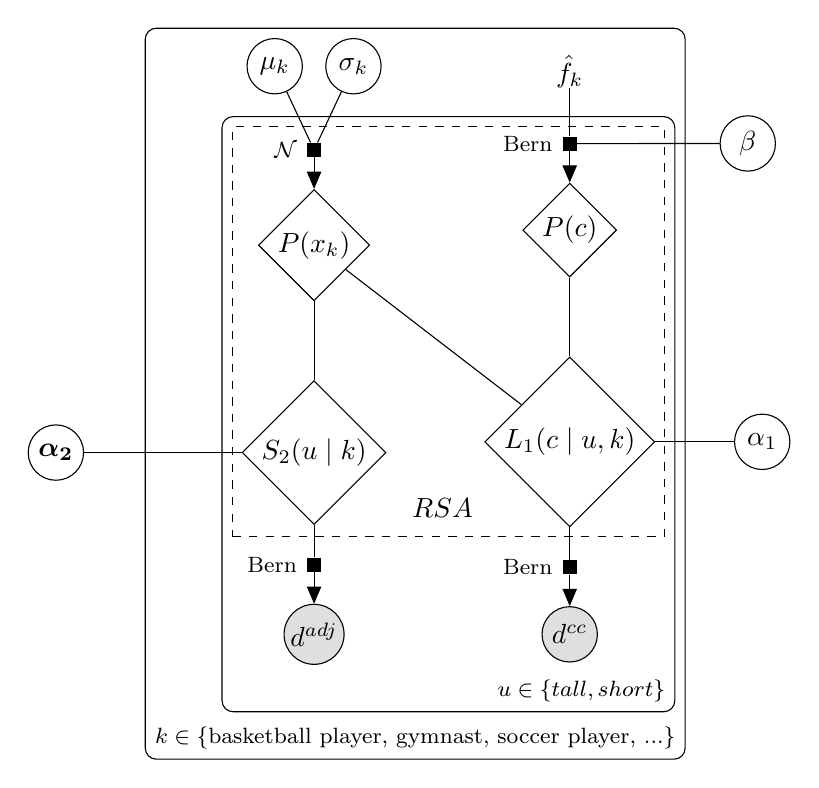
\begin{tikzpicture}


  % Y
  \node[obs]          (d-c)   {$d^{cc}$}; %
  \node[obs, left=2.5 of d-c]          (d-a)   {$d^{adj}$}; %
  \factor[above=of d-a] {da-f} {left:Bern} {} {} ; %
  \factor[above=of d-c] {dc-f} {left:Bern} {} {} ; %

  % W and X
  \node[det, above=of d-c] (L1) {$L_1(c \mid u, k)$} ; % 
  \node[det, above=of d-a] (S2) {$S_2(u \mid k)$} ; % 
  
%  \node[det, above right=1.2 of S2] (RSA) {RSA} ; % 
  
  \node[det, above=of S2]  (x)   {$P(x_k)$}; %
  \node[det, above=of L1] (c)   {$P(c)$}; %

  % C hyperpriors
   \node[const, above=1.2 of c] (fhat) {$\hat{f}_k$} ; %
   \node[latent, right=1.3 of c, yshift=1.1cm]  (b) {$\beta$} ; %
   \factor[above=of c] {c-f} {left:Bern} {fhat,b} {c} ; %

  % X hyperpriors
  \node[latent, above=1.2 of x, xshift=-0.5cm] (mx) {$\mu_k$} ; %
  \node[latent, above=1.2 of x, xshift=0.5cm]  (sx) {$\sigma_k$} ; %

  % sopt
   \node[latent, right=1cm of L1, yshift=0.0cm]         (a1)   {$\alpha_1$}; %
   \node[latent, left=2cm of S2]         (aa1)   {$\boldsymbol{\alpha_2}$}; %
%   \node[latent, left=2.5cm of S2, yshift=-0.6cm]         (aa2)   {$\alpha^{adj}_2$}; %
 % \node[const, above=of t, xshift=-0.5cm] (at)  {$\alpha_\tau$} ; %
  % \node[const, above=of t, xshift=0.5cm]  (bt)  {$\beta_\tau$} ; %

  % Factors
  \factor[above=of x] {x-f} {left:$\mathcal{N}$} {mx,sx} {x} ; %
%  \factor[above=of t] {t-f} {left:$\mathcal{G}$} {at,bt} {t} ; %
\factoredge {L1} {dc-f} {d-c} ; %
\factoredge {S2} {da-f} {d-a} ; %
%\factor       {W'-f}   {Multi} {} {};  %
  % Connect w and x to the dot node
  \edge[-] {c,x} {L1} ;
  \edge[-] {x} {S2} ;
%  \edge[-] {L1} {RSA} ;
%  \edge[-] {S2} {RSA} ;
  \edge[-] {a1} {L1} ;
%  \edge[-] {a1} {S2} ;
  \edge[-] {aa1} {S2} ;
%  \edge[-] {aa2} {S2} ;

\gate {RSAgate} {(L1)(S2)(x)(c)(x-f)(c-f)} {} ; %
\node[text width=1cm] at (-1.5,1.6) {$RSA$};
  % Plates
  \plate {P1} { %
  %  (d-c)(dc-f)(dc-f-caption) %
%    (x)(x-f)(x-f-caption) %
    %(RSA)
     (S2) (L1) (RSAgate)%
    (d-c)(d-a)%(x-f)
  } {$u \in \{tall, short\}$} ;
  \plate {yx} { %
  (P1)
    (d-c)(dc-f) %
    (x)(x-f)(mx)(sx)(fhat) %
    %(RSA) 
    (S2) (L1) %
  } {$k \in \{\text{basketball player, gymnast, soccer player, }...\}$} ;
  
    
%  \plate {} {%
%    (d-c)(dc-f)(dc-f-caption) %
%    (c)(da-f)(da-f-caption) %
%    (RSA) %
%    (yx.north west)(yx.south west) %
%  } {$M$} ;




%  % Define nodes
%  \node[latent]                             (u) {$u$};
%  \node[latent, above=of u, xshift=-1.2cm] (c) {${c}$};
%  \node[latent, above=of u, xshift=1.2cm]  (x) {${x}$};
%  \node[latent, above=of c, xshift=0cm] (f) {${f}$};
%  \node[latent, above=of x, xshift=0cm] (g) {${g}$};
%
%  % Connect the nodes
%  \edge {c,x} {u} ; %
%  \edge {f} {c} ; %
%  \edge {f,g} {x} ; %


\end{tikzpicture}

    \end{tabular}
  \end{center}
  \caption{Joint Bayesian data analytic strategy to infer model parameters and generate model predictions. Two similar RSA models (an adjective endorsement model $S_2$ and the comparison class inference model $L_1$) directly predict the data from Experiments 1 \& 2 ($d^{adj}$ and $d^{cc}$), respectively. Each of these models relies upon world knowledge $P(x_k)$ (e.g., prior expectations about the height of a basketball player), which are assumed to be Normal distributions with unknown mean $\mu_k$ and variance $\sigma_k$). The prior on comparison classes $P(c)$ is used only in the $L_1$ model, and is assumed to be a linear function of the log frequency of the noun phrase $\hat{f}_k$, with unknown scale parameter $\beta$. Each RSA model has its own set of speaker optimality parameters ($L_1$ has one parameter $\alpha_1$, while $S_2$ has two parameters $\boldsymbol{\alpha_2}$.}
  \label{fig:bayesnet}
\end{figure}





%To match the  we code the behavioral responses as to whether or not the mention the subordinate level category that is used to describe the referent in the experimental context. 
%
%
%Inferring the comparison class is necessarily a problem of inferring the intentions of another person.
%The relevant question is not \emph{is today a day in winter?} (an inference about the world), but rather \emph{did the speaker mean to draw a comparison to days to winter?} (an inference about intentions).
%Thus, a model for comparison class inference necessarily involves social reasoning about the speaker's intentions.
%
%Thus, the listener's beliefs about the temperature is a probability distribution conditional on the speaker and listener shared beliefs as well as the listener's private beliefs: $P(x \mid f, g)$.
%In the contexts we consider, the listener has no private beliefs and the totality of relevant shared beliefs boils down to the most specific categorization that the listener believes to be true of the referent (i.e., the day is a day in winter).

%On the other hand, on the shared beliefs $g$ can be used to guide 

%
%Both sets of beliefs can constrain the listener's belief distribution over the relevant degree as applied to the referent: If the listener knows that the day is a day in winter, they should use that information to guide their knowledge about the likely value of the degree $P(x \mid f, g)$.
%
%
%We model the scenario where a listener hears a gradable adjective describing a referent (e.g., that the temperature outside is warm) but does not know the comparison class assumed by the speaker. 
%To do this, a listener draws on their knowledge of the referent (e.g., that the day is a day in winter)
%
%When understanding vague language like a gradable adjective in context, a listener must integrate what they know about 
%
%Thus, we begin with a model for gradable adjective interpretation and build a mechanism for comparison class inference on top of this model. 
%. Where does this comparison class come from?
%
%We hypothesize that listeners maintain uncertainty about multiple
%possible comparison classes, but can reduce their uncertainty by
%combining world knowledge with pragmatic reasoning. More specifically,
%listeners use their world knowledge of what worlds are plausible under
%different comparison classes \(P(x \mid c)\) (e.g., the likelihood of
%different temperatures within different seasons), what implicit
%comparison classes are likely to be talked about \emph{a priori}
%\(P(c_i)\) (\(i\) for implicit), and how a rational speaker would behave
%in a given world assuming a particular comparison class
%\(S_{1}(u \mid x, c_i, \theta)\) (Eq. \ref{eq:L1a}). 
%
% As in previous models, we
%assume the listener is aware that the referent is a member of the
%subordinate class (and by extension, the superordinate as well). We
%additionally assume the pragmatic listener uses the most subordinate
%class information to inform the likely values of the degree (e.g., the
%listener's prior over temperatures is given by the distribution of
%temperatures for a specific class such as \emph{winter}
%\(P(x \mid c = c_{sub})\)). With these assumptions, the model becomes:
%
%\begin{align}
%L_{1}(x, c_{i}, \theta \mid u) &\propto S_{1}(u \mid x, c, \theta) \cdot P(x \mid c =  c_{sub}) \cdot P(c_{i}) \cdot P(\theta) \label{eq:L1a}\\
%S_{1}(u \mid x, c_i, \theta) &\propto \exp{(\alpha_1 \cdot \ln {L_{0}(x \mid u, c_i, \theta)}- \text{cost}(u)) } \label{eq:S1a}\\
%L_{0}(x \mid u, c_i, \theta) &\propto {\delta_{[\![u]\!](x, \theta)} \cdot P(x \mid \text{parseClass}(u, c_i))} \label{eq:L0a}
%\end{align}
%
%We are interested in the behavior of the pragmatic listener model with
%he hears an utterance without an explicit comparison class \(u_{i}\)
%(e.g., ``It's warm''). The listener reasons about alternative
%utterances the speaker could have said in order to draw pragmatic
%inferences. In this model, we assume the speaker has the option of
%conveying the adjective with an explicit comparison class \(u_{sub}\)
%and \(u_{super}\) (e.g., ``It's warm relative to other days in
%winter'' and ``It's warm relative to other days of the year'').
%The literal meanings of these alternatives are the same as the
%underspecified utterance (i.e., a threshold function:
%\([\![u_{warm}]\!] = x > \theta\)), but have the additional feature of
%overriding the implicit comparison class \(c_i\)and forcing the literal
%listener into a particular comparison class encoded in the utterance via
%the function \(\text{parseClass}\). That is:
%
%\begin{eqnarray}
%\text{parseClass}(u, c_i) & = &
%\begin{cases}
%c_{i} & \text{if } u = u_{i}\\
%c_{sub} & \text{if } u = u_{sub}\\
%c_{super} & \text{if } u = u_{super}\\
%\end{cases}
%\end{eqnarray}
%
%Thus, the speaker conditioning on a particular value for \(c_{i}\) only
%has implications for the literal listener if the speaker chooses to
%produce the implicit utterance (e.g., ``It's warm''). Should the
%speaker instead choose an utterance that explicitly articulates the
%comparison class (e.g., ``It's warm for winter''), the literal
%listener will use the explicit class to set his prior expectations
%\(P(x \mid c)\) via the \(\text{parseClass}\) operator.
%




%\subsubsection{Qualitative model predictions}


%\begin{figure*}[htb]

%{\centering 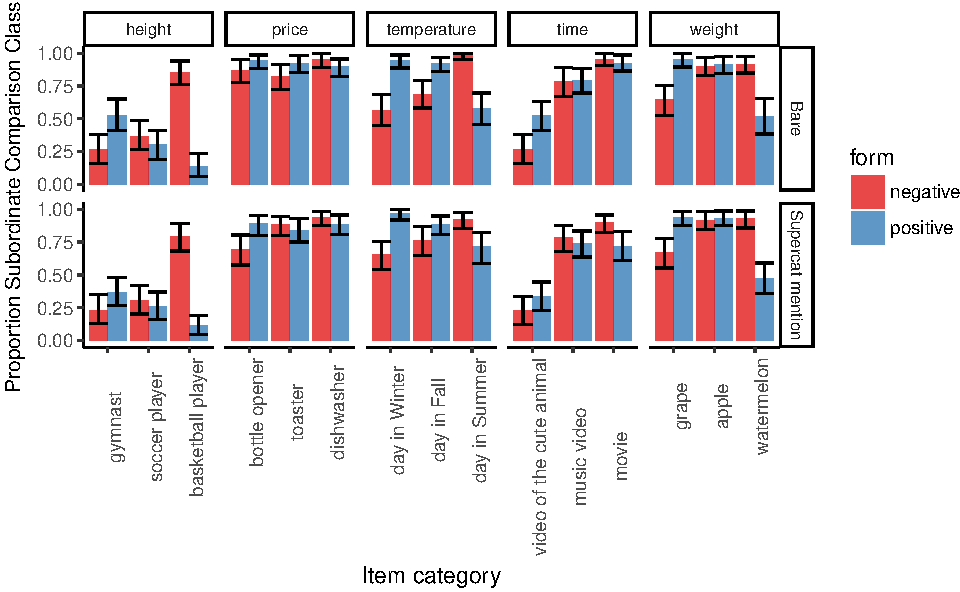
\includegraphics[width=1\textwidth]{figs/expt1results-1} 
%
%}
%
%\caption{Empirical comparison class judgments in terms of proportion in favor of subordinate comparison class.  Error bars correspond to 95\% Bayesian credible intervals.}\label{fig:expt1results}
%\end{figure*}
%
%\begin{figure*}[htb]
%
%{\centering \includegraphics[width=1\textwidth]{figs/modelParameters-1} 
%
%}

%\caption{Reconstructed degree priors (top) and empirically derived comparison class priors (botton). Top: Inferred prior distributions of world knowledge used to model Experiment 1 and 2 data. Bottom: Inferred prior probability of the subordinate comparison classes based on Google WebGram frequencies. Error bars correspond to 95\% Bayesian credible intervals, derived from the posterior on the $\beta$ scale parameter.}\label{fig:modelParameters}
%\end{figure*}

\section{Behavioral experiments}

We conduct three experiments to collect the data necessary to test the quantitative and quantitative predictions of our model, as outlined in Figure \ref{exptOverview}. 

\subsection{Step 1: Stimuli Generation}

\subsubsection{Participants}

We recruited 27 participants from Amazon's Mechanical
Turk and were restricted to those with U.S. IP addresses with at least a
95\% work approval rating. Each experiment took about 5 minutes and
participants were compensated \$0.60 for their work.

\subsubsection{Materials and procedure}

We used 8 pairs of positive- and negative-form gradable adjectives (Table \ref{tab:1}).
On each trial, participants were given a phrasal template, in which sentences that were missing subjects described the subjects as generally having the adjective apply (Figure \ref{fig:exptOverview}, Step 1). 
For example, ``\_\_\_ are generally big. \_\_\_ are generally small. \_\_\_ are sometimes big and sometimes small.'' These sentences were followed with another that made reference to the subjects that the participants filled-in: ``These three are all kinds of \_\_\_''. This last sentence was introduced to constrain the kinds of responses to the first three sentences such that the subjects would be all members of the same basic- or superordinate level category. 

\begin{table*}[ht]
\centering
\begingroup\fontsize{10pt}{11pt}\selectfont
\begin{tabularx}{\textwidth}{lll}
  \hline
Scale (adjectives) & Example subordinate classes (superordinate class) \\ 
  \hline
  \emph{big}, \emph{small} (size) & \\
\emph{tall}, \emph{short} (height) & \\ 
  \emph{expensive}, \emph{cheap} (price) & \\ 
    \emph{warm}, \emph{cold} (temperature) &  \\ 
  \emph{heavy}, \emph{light} (weight) &  \\ 
  \emph{long}, \emph{short} (duration / length) &  \\ 
  \emph{loud}, \emph{quiet} (loudness) &  \\ 
  \emph{light}, \emph{dark} (luminance) &  \\
   \hline
\end{tabularx}
\caption{Adjectives used in experiments.} 
\label{tab:1}
\endgroup
\end{table*}

\subsubsection{}


\subsection{Step 2: Adjective endorsement}

This experiment served to validate our experiment items generated in Step 1, as well as to provide further data that could be used to constrain the model parameters shown in Figure \ref{fig:bayesnet}.

\subsubsection{Procedure}

On each trial, participants were given a sentence introducing a member of a subordinate category (e.g., Alicia lives in Maryland and steps outside in winter.). 
This was followed by a question asking if the participant would endorse an adjective explicitly relative to the superordinate category (e.g., Do you think the day in winter would be warm relative to other days of the year?).
Participants could respond with either a \emph{yes} or \emph{no} judgment.

\subsubsection{Materials}

The experimental materials were a modified subset of those generated in Step 1. 
In addition to the sets of noun phrases forming the subordinate categories, a context sentence was crafted to provide an appropriate but minimal context in which the adjective could be uttered. 

\subsubsection{Results}

\subsection{Step 3: Comparison class inference}

\subsubsection{Procedure}

On each trial, participants were given a context sentence to introduce
the subordinate category (e.g., ``Tanya lives in Maryland and
steps outside in winter''). This was followed by an adjective sentence,
which predicated either a positive- or negative-form gradable adjective
over the item (e.g., ``Tanya says to her friend, ``It's
warm.''). Participants were asked ``What do you think Tanya
meant?'' and given a two-alternative forced-choice to rephrase the
adjective sentence with a freely-produced comparison class:

\begin{quote}
\{She / He / It\} is \textsc{adjective} (e.g., warm) relative to other \_\_\_\_.
\end{quote}

\begin{figure*}[htb]

{\centering \includegraphics{figs/posteriorPredictiveScatters-1} 

}

\caption{Human endorsement of subordinate comparison class paraphrases (middle; Expt. 1) and adjective sentences (left; Expt. 2) as a function of listener model $L_1$ and speaker model $S_2$ predictions, respectively. The right facet displays a subset of the paraphrase data (Expt. 1) to reveal good quantitative fit even in a small dynamic range. Error bars correspond to 95\% Bayesian credible intervals.}\label{fig:posteriorPredictiveScatters}
\end{figure*}

\subsubsection{Results}

We observed no systematic differences between participants' responses when the superordinate category was previously mentioned in the context and those when it was not; thus, we collapse across these two conditions for all analyses. Figure \ref{fig:expt1results} shows the proportion of participants choosing the \emph{subordinate} paraphrase for each item, revealing considerable variability both \emph{within}- and \emph{across}- scales. The predicted effects are visually apparent within each scale (compare with Figure \ref{fig:modelSchematics} right).

Our qualitative predictions are confirmed using a generalized linear mixed effects model with main effects of adjective form (positive vs.~negative) and the \emph{a priori} judgment by the first author of whether the sub-category was expected to be low or high on the degree scale, and of critical theoretical interest, the interaction between these two variables. In addition, we included by-participant random effects of intercept and by-subordinate category random effects of intercept and interaction between form and strength\footnote{This was the maximal mixed-effects structure that converged.}. Confirming our two qualitative model predictions, there was an interaction between form and strength (\(\beta = -3.82\); \(SE = 0.57;\) \(z = -6.73\)) and there was an overall preference for subordinate category paraphrases (\(\beta = 1.23\); \(SE = 0.45;\) \(z = 2.70\)). The main effects of form and strength were not significant.

We then test the simple effects. For items low on the degree scale (e.g., temperatures in winter), positive form adjectives were significantly more likely to imply subordinate comparison classes (\(\beta = 1.41\); \(SE = 0.15;\) \(z = 9.43\)), while the opposite is true for items high on the scale (e.g., summer days; \(\beta = -2.50\); \(SE = 0.19;\) \(z = -13.15\)). Participants reason pragmatically to resolve the comparison class, combining world knowledge with informativity as predicted by our model.

\subsection{Quantitative modeling}


The full model's posterior over the RSA and data-analytic parameters were consistent with prior literature and intuition. The maximum a-posteriori (MAP) estimate and 95\% highest probability density (HPD) intervals for model parameters specific to the \(L_1\) model used for comparison class inference were \(\alpha^{1}_{1} = 1.60 [1.10, 2.50]\), \(\beta = 0.13 [0.11, 0.19]\). Model parameters specific to the \(S_2\) model used for adjective endorsement: \(\alpha^{2}_{1} = 3.50 [0.60, 13.20]\), \(\alpha^{2}_{2} = 3.20 [2.60, 3.80]\). The inferred distributions corresponding to subordinate class priors were consistent with the \emph{a priori} ordering of these subordinate classes (low, medium, high) used in these tasks (Figure \ref{fig:modelParameters} top).

Finally, the full model's posterior predictive distribution does an excellent job at capturing the quantitative variability in comparison class inferences: \(r^2(30) = 0.96\), and adjective endorsements: \(r^2(30) = 0.98\) (Figure \ref{fig:posteriorPredictiveScatters}). Because of the overall preference for the subordinate comparison class, many of the data points are distributed above 0.5. Even for these fine-grained differences, the model does a good job at explaining the quantitative variability in participants' data (Figure \ref{fig:posteriorPredictiveScatters} right). Thus, the variability in comparison class inferences we observe in our behavioral data can be accounted for the constructs posited in our model (namely, the comparison class prior and degree priors).

\section{Discussion}

Investigations of how human listeners understand vague adjectives have
shed light on the precise mechanisms by which people interpret
context-sensitive language, but have had little to say about how
listeners decide upon what counts as the appropriate context. In this
paper, we take the first step towards investigating the flexibility in
the class against which an entity can be implicitly compared, a very
basic form of context. We introduced a minimal extension to an adjective
interpretation Rational Speech Act model to allow it to flexibly reason
about the comparison class. This model made the novel prediction that
listeners should try to accomodate a vague utterance by choosing the
comparison class most likely to make the utterance true while
prioritizing more specific (lower variance) classes because they are
more informative. It also made quantitative predictions about how
background knowledge about the degree scale and what classes are likely
to be talked about \emph{a priori} should inform this inference in a
graded fashion. Both qualitative predictions of the model were borne out
in our behavioral experiment, and the quantitative predictions were
confirmed using a novel data analytic technique.

Resolving underspecification by means of a comparison is not unique to
\emph{gradable adjectives} like ``big'' or ``tall'', but is
a general problem for language understanding. ``John ate \emph{a
lot} of hot dogs'' probably means four or five hot dogs, whereas
``John ate \emph{a lot} of potato chips'' could imply a quantity
over a hundred (Schöller \& Franke, 2017); ``Robins lay eggs''
means roughly that \emph{female robins} lay eggs, whereas
``Robins fly'' entails something stronger, most or all robins fly
({\textbf{???}}; {\textbf{???}}). Even noun concepts (e.g.,
``furniture'') are graded (Rosch \& Mervis, 1975) and can be made
more precise in context. Investigating how listeners interpret words
like ``big'' is thus a case study of a crucial, general problem in
language understanding: Understanding context-sensitive language.

We investigated the question of how a listener decides among multiple
possible conceptually-based comparison classes (e.g., tall for a
basketball player vs.~tall for a person). It is notable that our model
was able to account for inferences about items that did not fall into
strict hierachies (e.g., \emph{movies} is not subordinate to
\emph{things you watch online}) as well as items that did (e.g.,
basketball players and people). This result suggests that our modeling
framework can easily extend into cross-cutting comparison classes (e.g.,
\emph{men}, \emph{people of a certain age}, \emph{basketball players}).

\subsection{The phenomenon of comparison class
inference}

To our knowledge, we present the first behavioral data of how reference
classes for adjective interpretation can adjust based on world
knowledge. Previous experimental work on adjective understanding in
young children has looked at what counts as being in the comparison
class (e.g., the comparison class for a ``tall pimwit'' is \emph{other
pimwits} and not \emph{other creatures in general}; Barner \& Snedeker,
2008) or how flexibly children can shift between different kinds of
comparison classes (Ebeling \& Gelman, 1994), but now the factors that
determine the comparison class. We demonstrate one such factor: world
knowledge.

It's been suggested that there exist qualitatively different kinds of
comparison classes, constructed by reference to either: the perceptual
context (a \emph{perceptual comparison class}), a goal of an agent or
intended use of an object (a \emph{functional comparison class}), and
the kind of the referent (a \emph{conceptual comparison class}; Ebeling
\& Gelman, 1994). In this paper, we investigated the latter, but the
question remains about how a listener should decide to switch between
different kinds of comparison classes. For example, if Ann and Carl are
deciding what to do on a Friday night, and Ann offers ``The
ballet is expensive'', Carl should interpret not as a statement relative
to \emph{other ballets} or either \emph{other forms of entertainment},
but to \emph{other ways Ann and Carl could spend their Friday night}, a
functional comparison class. Goal inference is thus an associated
ingredient in comparison class inference, and integrating the two
should be a target for future work.

The syntactic frame in which the adjective manifests also appears to
vary how strongly the noun phrase constrains the comparison class. In
our experiment, we used syntatically minimal frames (e.g., ``He's
tall''). A speaker who explicitly articulates a noun for the referent
(e.g., ``That basketball player is tall'', especially with
prosodic focus on ``that'') could reveal how she is
conceptualizing the referent and thus provide a strong cue to the
comparison class. Prenominal uses of the adjective (e.g., ``He's
a tall basketball player'') might be an even stronger cue. Prenominal
uses are considered the ideal form for a child learning the meaning of
novel adjectives ({\textbf{???}}; {\textbf{???}}; {\textbf{???}}),
perhaps because it is such a strong cue to the comparison class.

\subsection{Comparison class prior}

We observe in our quantitative modeling results that a uniform prior
distribution over the experimentally supplied comparison class
alternatives is unlikely (Figure \ref{fig:modelParameters} bottom). For
example, the comparison class of ``people'' for heights of
individuals is relatively more salient than the class of
``produce'' (or, ``fruits and vegetables'') for the weights
of particular fruits and vegetables. We used the frequency of the class
in a corpus as a proxy for their prior probability \(P(c)\), which was
sufficient to account for differences in baseline class probability both
\emph{between}- and \emph{within}-scales.

Corpus frequency is a composite measurement of factors relevant for
speech production. Its utility in this model suggests that utterances
without an explicit comparison class (e.g., ``It's warm outside'')
may in fact be incomplete sentences, in a way analogous to sentence
fragments studied in noisy-channel models of production and
comprehension (Bergen \& Goodman, 2015). Another (non-mutually
exclusive) possibility is that the comparison class prior reflects
basic-level effects in categorization (Rosch \& Mervis, 1975). Future
work should attempt to understand these factors to construct a more
complete theory of the comparison class prior.

\subsection{Fully Bayesian analysis of Bayesian language
models}

The second contribution of this paper is a novel data-analytic approach,
where prior knowledge used in the Bayesian language model is
reconstructed from converging evidence gathered from a related language
experiment, also explicitly modeled using a language understanding
model. In previous work, we have attempted to measure prior knowledge by
decomposing what would be a single, implicitly multilayered, numerical
estimation question into multiple simpler questions. Then, we construct
a Bayesian data analytic model to back out the prior knowledge (Tessler
\& Goodman, 2016a, 2016b). We extend this approach by using the same
core RSA model to model behavior across two language experiments. The
major feature of this method is that participants respond only to
simple, natural language questions rather than estimating numerical
quantities for which complicated linking functions must be designed
(e.g., Franke et al., 2016). The fully Bayesian language approach we
pioneer here also provides a further constraint on the language model,
which must predict data from two similar but distinct language
experiments. The productivity of natural language can thus be harnessed
to productively design experiments that further constrain and test
computational models of language and cognition.

\section{Conclusion}

The words we say are often too vague to have a single, precise meaning,
and only make sense in context. The context, however, can also be
underspecified, leaving the listener in the dark about both the
speaker's intended meaning and about the context through which the
listener is to make sense of the conversation. This work suggests,
however, that listeners are able to jointly infer a lot from a little:
The meaning and the context from a single vague utterance.


\section{Acknowledgements}

This work was supported in part by NSF Graduate Research Fellowship
DGE-114747 to MHT, a Stanford CSLI Summer Internship for MLB, and a
Sloan Research Fellowship, ONR grant N00014-13-1-0788, and DARPA grant
FA8750-14-2-0009 to NDG.

\newpage


\bibliographystyle{apacite}

%\setlength{\bibleftmargin}{.125in}
%\setlength{\bibindent}{-\bibleftmargin}

\bibliography{comparison-class}

\newpage
\section{Appendix}


%Gradable adjectives like \emph{warm} and \emph{cold} are vague
%descriptions of an underlying quantitative scale (e.g., temperature).
Classic semantic theories posit the meaning of gradable adjectives to simply be that the scalar degree $x$ (e.g., temperature) is greater than or less than a contextually-supplied standard of comparison  \(\theta_c\): \([\![u_{pos}]\!] = x > \theta_c\), for positive-form adjectival utterance \(u_{pos}\) (e.g., warm) and \([\![u_{neg}]\!] = x < \theta_c\), for negative-form adjectival utterance \(u_{neg}\) (e.g., cold).
 Lassiter \& Goodman (2013) model the context-sensitivity of these adjectival utterances using threshold semantics, where
the threshold is probabilistically set with respect to a comparison class \(c\) via pragmatic reasoning :

\begin{align}
L_{1}(x, \theta \mid u, c) &\propto S_{1}(u \mid x, \theta) \cdot P(x \mid c) \cdot P(\theta) \label{eq:L1} \\
S_{1}(u \mid x, \theta, c) &\propto \exp{(\alpha_1 \cdot (\ln {L_{0}(x \mid u, \theta, c)} - \text{cost}(u)))} \label{eq:S1}\\
L_{0}(x \mid u, \theta, c) &\propto {\delta_{[\![u]\!](x, \theta)} \cdot P(x \mid c)} \label{eq:L0}
\end{align}

Eqs. \ref{eq:L1} - \ref{eq:L0} are the Rational Speech Act mode  Lassiter \& Goodman (2013). 
In this model, a pragmatic listener \(L_1\)
tries to resolve the degree \(x\) (e.g., the temperature)
from the adjectival utterance she heard \(u\) (e.g., ``it's warm''), by assuming the utterance came from an approximately rational Bayesian
speaker \(S_1\) trying to inform a naive listener \(L_0\), who in turn
updates their prior beliefs \(P_c(x)\) via an utterance's literal meaning
\([\![u]\!](x, \theta)\).
Formally, the literal meaning is represented by the
Kronecker delta function \(\delta_{\mbox{ $[\![ u ]\!]$}(x, \theta)}\)
that returns probabilities proportional to \(1\) when the utterance is
true (i.e., when \(x > \theta\)) and \(0\) otherwise.
The key innovation used for modeling gradable adjectives is to have uncertainty over the
semantic variable---the threshold \(\theta\) (Eq. \ref{eq:L1}). In
Lassiter and Goodman (2013)'s model, \(\theta\) comes from an improper uniform
prior distribution over thresholds defined over the real numbers and is resolved by the
listener reasoning about the different thresholds a speaker might be
using \(S_{1}(u \mid x, \theta)\) as well as the probabilities of
different states of the world \(P(x \mid c)\) (e.g., different
temperatures). Assuming the adjective adds some cost to the speaker's
utterance (Eq. \ref{eq:S1}), the meaning of a gradable adjectives (e.g.,
``warm'') is resolved by the pragmatic listener to mean something
like ``significantly greater temperature than one might expect''
(Lassiter \& Goodman, 2015). Critically, what ``one might
expect''---the prior distribution over temperatures \(P(x \mid c)\)---is
always with respect to some comparison class \(c\) (Eqs. \ref{eq:L1} \&
\ref{eq:L0})


\end{document}
